% !TEX root = main.tex
\subsubsection{Contextual bandits not in the exponential family}
\label{sssec:evaluation_mixture_scenarios_baselines}

We now study a set of more challenging contextual MABs, \ie those where the underlying reward distributions do not fit into the exponential family assumption.
Specifically, we study the following contextual bandit scenarios, where the context is randomly drawn from a two dimensional uniform distribution, \ie $x_{i,t}\sim\U{0,1}$, $i\in\{0,1\}$, $t\in \Natural$.

\texttt{Scenario A:}
\begin{equation}
\begin{cases}
p_{1}(y|x_t,\theta) = 0.5 \cdot \N{y|x_t^\top(0 \; 0), 1} + \; 0.5 \cdot \N{y|x_t^\top(1 \; 1), 1}\\
p_{2}(y|x_t,\theta) = 0.5 \cdot \N{y|x_t^\top(2 \; 2), 1} + \; 0.5 \cdot \N{y|x_t^\top(3 \; 3), 1}
\end{cases}
\nonumber
\end{equation}
\texttt{Scenario B:}
\begin{equation}
\begin{cases}
p_{1}(y|x_t,\theta) = 0.5 \cdot \N{y|x_t^\top(1 \; 1), 1} + \; 0.5 \cdot \N{y|x_t^\top(2 \; 2), 1}\\
p_{2}(y|x_t,\theta) = 0.3 \cdot \N{y|x_t^\top(0 \; 0), 1} + \; 0.7 \cdot \N{y|x_t^\top(3 \; 3), 1}
\end{cases}
\nonumber
\end{equation}
\texttt{Scenario C:}
\begin{equation}
\begin{cases}
p_{1}(y|x_t,\theta) = \N{y|x_t^\top(1 \; 1), 1}\; ,\\
p_{2}(y|x_t,\theta) = 0.5 \cdot \N{y|x_t^\top(1 \; 1), 1} + \; 0.5 \cdot \N{y|x_t^\top(2 \; 2), 1}\\
p_{3}(y|x_t,\theta) = 0.3 \cdot \N{y|x_t^\top(0 \; 0), 1} + \; 0.6 \cdot \N{y|x_t^\top(3 \; 3), 1} + \; 0.1 \cdot \N{y|x_t^\top(4 \; 4), 1} 
\end{cases}
\nonumber
\end{equation}
\texttt{Scenario D:}
\begin{equation}
\begin{cases}
p_{1}(y|x_t,\theta) = 0.75 \cdot \N{y|x_t^\top(0 \; 0), 1} + \; 0.25 \cdot \N{y|x_t^\top(0 \; 0), 10} \\
p_{2}(y|x_t,\theta) = 0.75 \cdot \N{y|x_t^\top(2 \; 2), 1} + \; 0.25 \cdot \N{y|x_t^\top(2 \; 2), 10}
\end{cases}
\nonumber
\end{equation}

The reward distributions of these contextual bandits are all Gaussian mixtures, which differ in the amount of mixture overlap and the similarity between arms.
In these scenarios, the reward functions are not within the exponential family of distributions: they are all multi-modal, unbalanced in \texttt{Scenarios B} and \texttt{C}, and with heavy tails in \texttt{Scenario D}.

\texttt{Scenario A} is a balanced mixture of two Gaussian distributions, with rewards easily separable per-arm.
On the contrary, there is a significant overlap between arm rewards in \texttt{Scenario B}, with quite unbalanced mixtures for arm 2: rewards from a mixand of low expected value are drawn with probability $0.3$, and higher rewards are expected with probability $0.7$.
\texttt{Scenario C} describes a MAB with different per-arm reward distributions: a linear Gaussian distribution for arm 1, a bi-modal Gaussian mixture for arm 2, and an unbalanced Gaussian mixture with three components for arm 3.
Finally, \texttt{Scenario D} models heavy-tailed distributions, where the bandit is subject to outlier rewards.

We show in Figure~\ref{fig:mixture_scenarios_bandit_showdown_baselines} how our proposed method adjusts to the underlying reward model complexity, attaining reduced cumulative regret when compared to other Thompson sampling-based alternatives, in all the studied scenarios.

% Mixture bandit regret figure (moved here so that it appears soon in text)
\begin{figure*}[!ht]
	\centering
	\begin{subfigure}[c]{0.45\textwidth}
		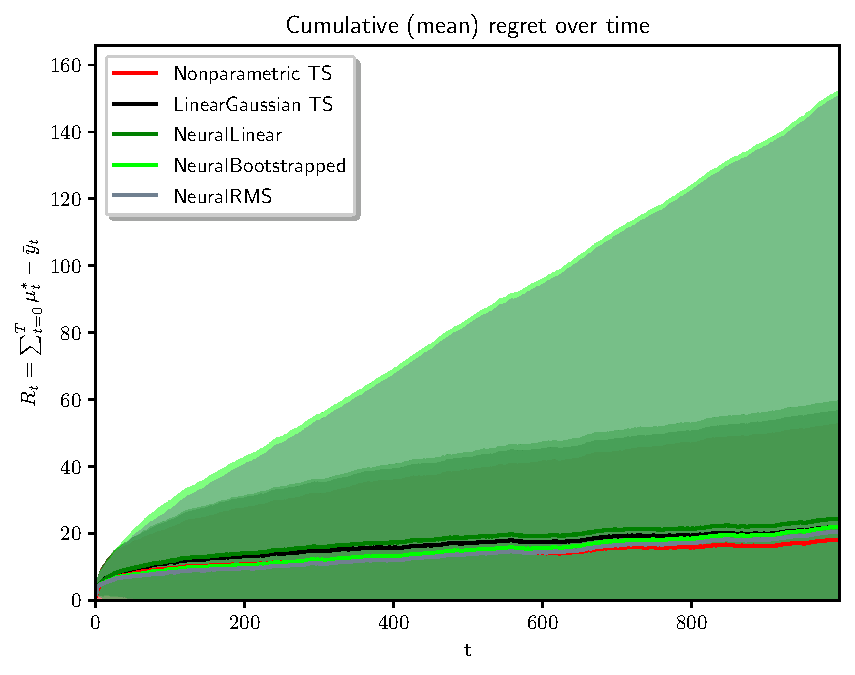
\includegraphics[width=\textwidth]{./figs/linear_gaussian_mixture_easy_baselines/cum_optexpected_regret_top_five_std}
		\vspace*{-5ex}
		\caption{\texttt{Scenario A}.}
		\label{fig:scenario_A_baselines_top}
	\end{subfigure}
	\begin{subfigure}[c]{0.45\textwidth}
		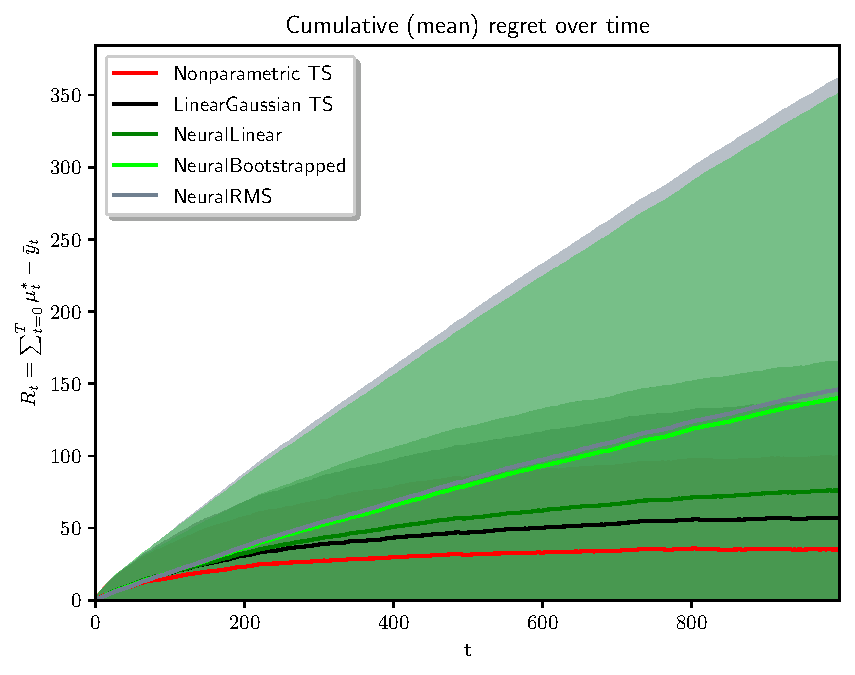
\includegraphics[width=\textwidth]{./figs/linear_gaussian_mixture_hard_baselines/cum_optexpected_regret_top_five_std}
		\vspace*{-5ex}
		\caption{\texttt{Scenario B}.}
		\label{fig:scenario_B_baselines_top}
	\end{subfigure}
	
	\begin{subfigure}[c]{0.45\textwidth}
		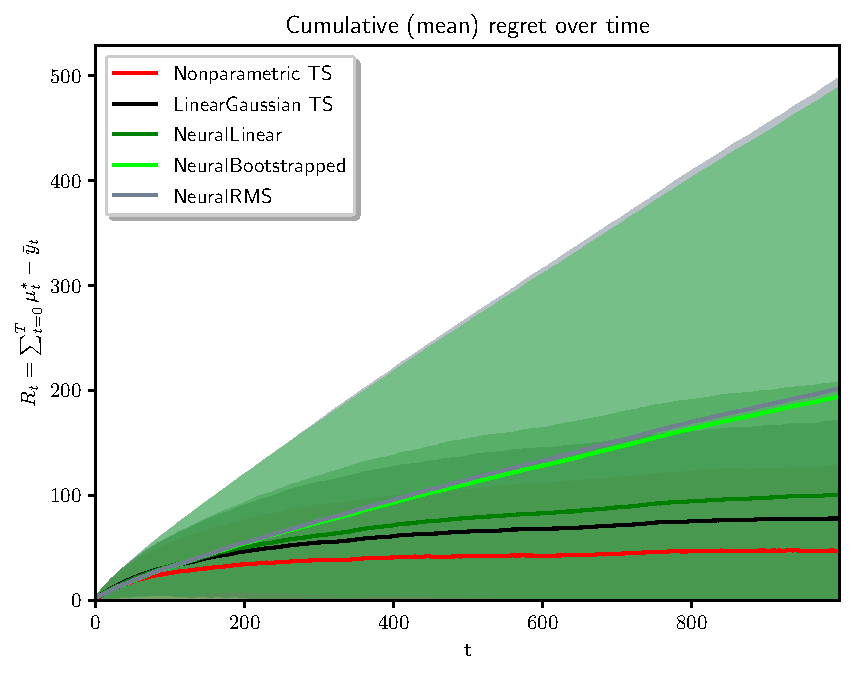
\includegraphics[width=\textwidth]{./figs/linear_gaussian_mixture_unbalanced_baselines/cum_optexpected_regret_top_five_std}
		\vspace*{-5ex}
		\caption{\texttt{Scenario C}.}
		\label{fig:scenario_C_baselines_top}
	\end{subfigure}
	\begin{subfigure}[c]{0.45\textwidth}
		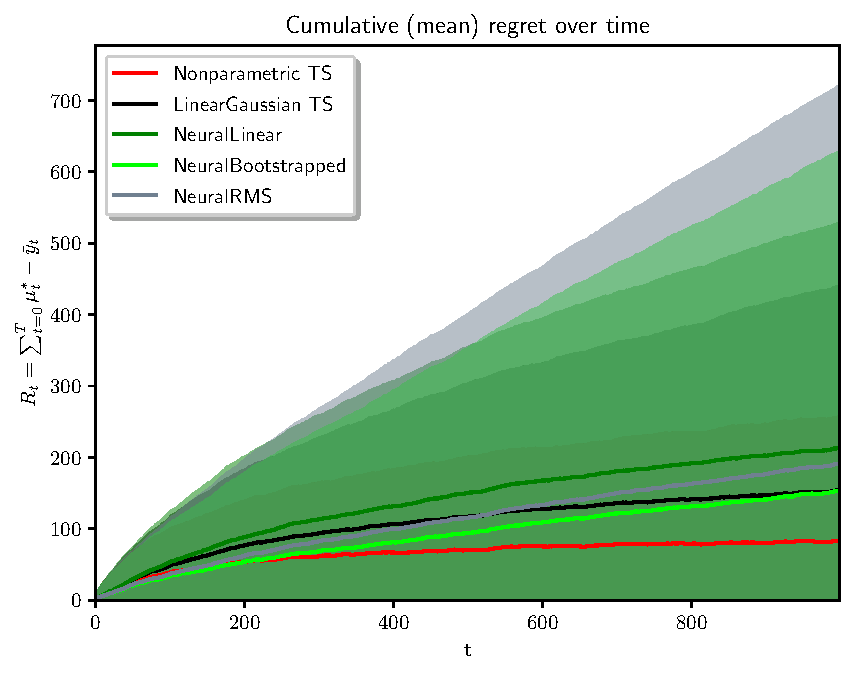
\includegraphics[width=\textwidth]{./figs/linear_gaussian_mixture_heavy_tail_baselines/cum_optexpected_regret_top_five_std}
		\vspace*{-5ex}
		\caption{\texttt{Scenario D}.}
		\label{fig:scenario_D_baselines_top}
	\end{subfigure}
	\vspace*{-2ex}
	\caption{Mean cumulative regret (standard deviation shown as shaded region) for $R=500$ realizations of the top-performing methods in all studied scenarios.}
	\label{fig:mixture_scenarios_bandit_showdown_baselines}
\end{figure*}

% Mixture bandit regret table
\begin{table*}[!ht]
	\caption{Mean cumulative regret at $t=1000$ for $R=500$ realizations of the studied methods in all scenarios. We indicate in parentheses the additional relative cumulative regret incurred by each algorithm when compared to \texttt{Nonparametric TS}.}
	\label{tab:mixture_scenarios_bandit_showdown_baselines_regret}
	\vspace*{-4ex}
	\begin{center}
		\resizebox*{\textwidth}{!}{
			\begin{tabular}{|c|c|c|c|c|}
				\hline
				Algorithm 	\cellcolor[gray]{0.6} & \texttt{Scenario A} \cellcolor[gray]{0.6} & \texttt{Scenario B} \cellcolor[gray]{0.6} & \texttt{Scenario C} \cellcolor[gray]{0.6} & \texttt{Scenario D} \cellcolor[gray]{0.6} \\ \hline
				Nonparametric TS       	& 18.105	 (\%0.000)	&	35.268	 (\%0.000)		&	47.172	 (\%0.000)		&	83.464	 (\%0.000) \\ \hline
				LinearGaussian TS      	& 21.957	 (\%21.276)	&	57.04	 (\%61.733)		&	77.921	 (\%65.184)		&	153.955	 (\%84.456) \\ \hline
				NeuralLinear           	& 24.358	 (\%34.538)	&	76.312	 (\%116.377)	&	100.202	 (\%112.415)	&	213.073	 (\%155.286) \\ \hline
				NeuralBootstrapped     	& 21.942	 (\%21.195)	&	140.302	 (\%297.816)	&	194.198	 (\%311.676)	&	153.315	 (\%83.690) \\ \hline
				NeuralRMS              	& 20.559	 (\%13.551)	&	146.276	 (\%314.756)	&	201.818	 (\%327.829)	&	191.552	 (\%129.501) \\ \hline
				NeuralDropoutRMS       	& 26.191	 (\%44.663)	&	146.182	 (\%314.490)	&	202.297	 (\%328.846)	&	170.3	 (\%104.039) \\ \hline
				NeuralParamNoise       	& 23.17	 	 (\%27.976)	&	129.758	 (\%267.921)	&	170.385	 (\%261.197)	&	177.931	 (\%113.182) \\ \hline
				MultitaskGP            	& 114.79	 (\%534.020)&	145.883	 (\%313.643)	&	245.441	 (\%420.305)	&	667.407	 (\%699.631) \\ \hline
				BNNVariationalGaussian  & 27.643	 (\%52.682)	&	172.461	 (\%389.001)	&	217.891	 (\%361.903)	&	340.92	 (\%308.462) \\ \hline
				BNNAlphaDiv            	& 67.969	 (\%275.416)&	196.028	 (\%455.824)	&	306.14	 (\%548.980)	&	247.998	 (\%197.130) \\ \hline
			\end{tabular}
		}
	\end{center}
	\vspace*{-4ex}
\end{table*}

In \texttt{Scenario A}, even if all shown methods attain logarithmic regret (\ie they are able to find the right exploitation-exploration balance) as shown in Figure~\ref{fig:scenario_A_baselines_top}, our proposed method attains meaningful regret reductions.
The attained cumulative regret results (with relative regret improvements) are detailed in Table~\ref{tab:mixture_scenarios_bandit_showdown_baselines_regret}, and the corresponding reward results are provided in Section~\ref{asec:mixture_baselines} of the Appendix.

In \texttt{Scenario A}, the second best performing \texttt{NeuralRMS} baseline incurs an additional 13.5\% cumulative regret when compared to \texttt{Nonparametric TS}, \texttt{LinearGaussian TS} is 21.3\% worse, and a regret increase of 21.2\% and 34.5\% is observed for the \texttt{NeuralBootstrapped} and \texttt{NeuralLinear} baselines, respectively.

\texttt{Nonparametric TS} provides important regret savings when compared to the best performing alternative in each scenario:
at least an additional 61.7\%, 65.2\% and 83.69\% cumulative regret is incurred by other baselines at the end of \texttt{Scenario B}, \texttt{Scenario C}, and \texttt{Scenario D}, respectively.
The proposed Bayesian nonparametric mixture model Thompson sampling clearly outperforms all the alternatives in the studied scenarios.
Besides, the volatility in regret performance of \texttt{Nonparametric TS} is the smallest of all the studied alternatives across all scenarios.

Even if each scenario is a different MAB setting, \texttt{Nonparametric TS} is readily applicable to all, without any per-case specific fine-tuning:
even in \texttt{Scenario C}, where there are different model classes per-arm.
Overall, \texttt{Nonparametric TS} attains reduced regret in all the studied MABs ---with different unknown per-arm distributions not in the exponential family.

On the contrary, we observe a poor performance of neural network and approximate Bayesian inference based alternatives.
Specifically, we find that the linear neural alternative takes longer to reach the exploration-exploitation tradeoff.
\citet{ip-Riquelme2018} argued that \texttt{NeuralLinear} is able to simultaneously learn a good latent data representation, and to accurately quantify the uncertainty over linear models, to explain the observed rewards in terms of these learned representation. This competitive advantage allowed~\citet{ip-Riquelme2018} to successfully solve problems that require non-linear representations where linear approaches fail. However, we here observe a significant regret increase in comparison to our proposed nonparametric method for bandits with reward functions not in the exponential family:
additional 34.54\%, 116.377\%, 112.415\% and 155.29\% regret is incurred in \texttt{Scenarios A}, \texttt{B}, \texttt{C}, and \texttt{D}, respectively.

In addition, bootstrapped and RMS based neural Thompson sampling techniques struggle to find a good exploration-exploitation balance, incurring in additional (and very volatile) regret performance, as shown in Figure~\ref{fig:mixture_scenarios_bandit_showdown_baselines}.
As noted by~\citet{ip-Riquelme2018}, ($i$) bootstrapping incurs in a heavy computational overhead, depending on the number of networks considered; ($ii$) a noise-injection based method is hard to tune and sensitive to the heuristic controlling the injected noise-level; and ($iii$) dropout algorithms heavily depend on their hyperparameters, and it is unclear how to disentangle better training from better exploration in these models. On the contrary, \texttt{Nonparametric TS} achieves reduced regret across all scenarios without any case-specific fine-tuning.

Alternative nonparametric methods, such as those based on Gaussian processes also suffer in all the studied scenarios (see Table~\ref{tab:mixture_scenarios_bandit_showdown_baselines_regret}). We argue that the low performance of this method is explained by model misspecification: Gaussian process regression methods require knowledge of the true underlying model class (\ie what mean and kernel functions to use) ---if the reward model class of the MAB they are targeting is not correctly specified, then increased regret is attained. Note that, in \texttt{Nonparametric TS}, no per-MAB fine tuning is required.

Variational inference and expectation-propagation based algorithms also perform poorly in all the studied scenarios (see Table~\ref{tab:mixture_scenarios_bandit_showdown_baselines_regret}). As reported by~\citet{ip-Riquelme2018}, while optimizing to convergence at every interaction with the world incurs increased computational cost, results suggest that it may not be sufficient to partially optimize the variational parameters in bandit settings. Similarly, for Black-Box $\alpha$-divergence, partial convergence may be the cause of poor performance. Overall, there is a need for investigating how to sidestep the slow convergence of the uncertainty estimates in bandit settings for these neural network based methods.

The volatility of all the evaluated neural network based alternatives is noteworthy, and worrisome: their performance is highly variable when compared to the proposed nonparametric method (reward standard deviation details are provided in Section~\ref{asec:mixture_baselines} of the Appendix.).

On the contrary, the performance of \texttt{Nonparametric TS} is much less volatile.
For real-life bandit applications, the variance of an algorithm's performance is critical: even if expected reward guarantees are in place, the understanding of how volatile a bandit algorithm's decisions are, has undeniable real-world impact.

All in all, we conclude that our proposed nonparametric Thompson sampling outperforms (both in averaged cumulative regret, and in regret volatility) other alternatives across all the studied scenarios. Due to the capacity of Bayesian nonparametrics to autonomously adjust the complexity of the model to the sequentially observed data, the proposed method can, without any per-scenario tuning ($Gibbs_{max}=10$, $d_a=0$, $\gamma_a=0.1$, $\forall a$, in all the experiments), readily target all of them, and attain considerable regret reductions.

Important savings are achieved for MAB settings not in the exponential family (\ie unbalanced and heavy tailed distributions) and for bandits with different per-arm reward distributions, where we observe that alternative methods struggle.
The competitive advantage lies on the capacity of Bayesian nonparametrics to adjust the complexity of the posterior density to the sequentially observed bandit data. 

% Gibbs
\begin{figure*}[!h]
	\centering
	\begin{subfigure}[c]{0.45\textwidth}
		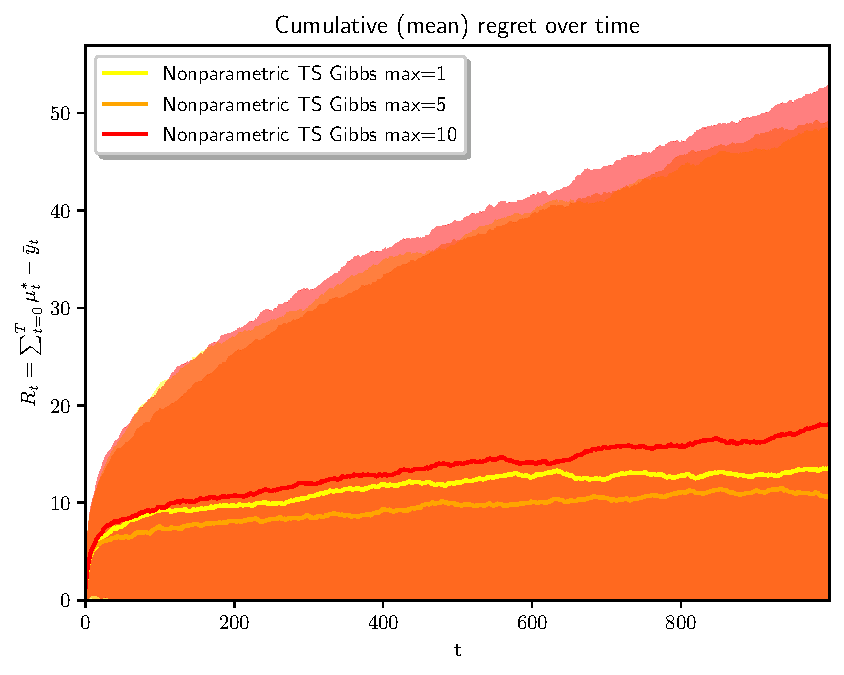
\includegraphics[width=\textwidth]{./figs/linear_gaussian_mixture_easy_gibbsmaxiter/cum_optexpected_regret_top_five_std}
		\vspace*{-5ex}
		\caption{\texttt{Scenario A}.}
		\label{fig:scenario_A_gibbsmaxiter_std}
	\end{subfigure}
	\begin{subfigure}[c]{0.45\textwidth}
		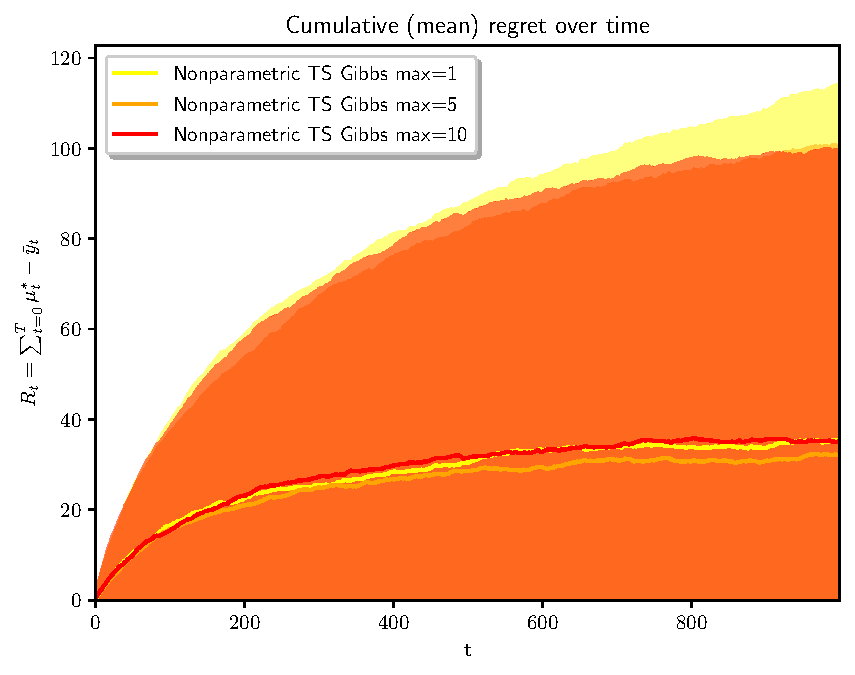
\includegraphics[width=\textwidth]{./figs/linear_gaussian_mixture_hard_gibbsmaxiter/cum_optexpected_regret_top_five_std}
		\vspace*{-5ex}
		\caption{\texttt{Scenario B}.}
		\label{fig:scenario_B_gibbsmaxiter_std}
	\end{subfigure}
	
	\begin{subfigure}[c]{0.45\textwidth}
		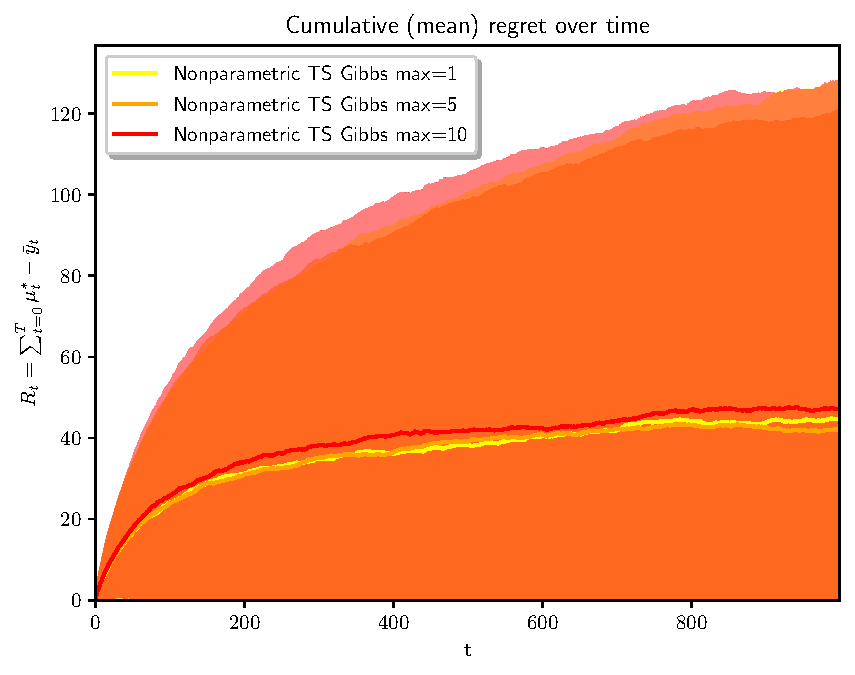
\includegraphics[width=\textwidth]{./figs/linear_gaussian_mixture_unbalanced_gibbsmaxiter/cum_optexpected_regret_top_five_std}
		\vspace*{-5ex}
		\caption{\texttt{Scenario C}.}
		\label{fig:scenario_C_gibbsmaxiter_std}
	\end{subfigure}
	\begin{subfigure}[c]{0.45\textwidth}
		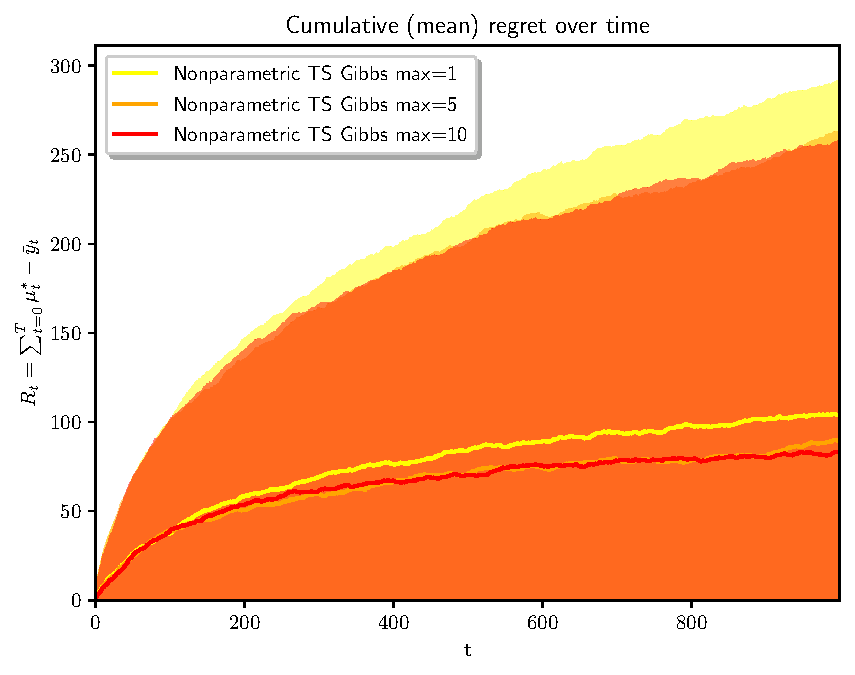
\includegraphics[width=\textwidth]{./figs/linear_gaussian_mixture_heavy_tail_gibbsmaxiter/cum_optexpected_regret_top_five_std}
		\vspace*{-5ex}
		\caption{\texttt{Scenario D}.}
		\label{fig:scenario_D_gibbsmaxiter_std}
	\end{subfigure}
	\vspace*{-2ex}
	\caption{Mean regret (standard deviation shown as shaded region) for $R=500$ realizations of the proposed \texttt{Nonparametric TS} method with different $Gibbs_{max}$ in all scenarios.}
	\label{fig:mixture_scenarios_bandit_showdown_gibbsmaxiter}
\end{figure*}

Finally, we investigate the \textit{warm-start} effect in the proposed algorithm's Gibbs sampling procedure, and how the practical recommendations on limiting the number of Gibbs iterations of Section~\ref{sssec:nonparametric_thompson_sampling_computational_complexity} impact regret performance.

In general, and because of the incremental availability of observations in the bandit setting, we observe that the proposed Gibbs sampler achieves quick convergence: in all our experiments, a 1\% log-likelihood relative difference between iterations is usually achieved within $Gibbs_{max}\leq10$ iterations.
We show in Figure~\ref{fig:mixture_scenarios_bandit_showdown_gibbsmaxiter} that no significant regret performance improvement is achieved by letting the sampler run for a high number of iterations. 

\textit{A good enough} posterior convergence at a limited computational budget ---at most $Gibbs_{max}$ updates over all $t_a$ observations for the played arm--- is possible because the Gibbs sampler is run, at each interaction with the world, from a good starting point: the per-arm parameter space that describes all but this newly observed reward.

Therefore, when computational constraints are appropriate, \eg for real-time bandits, limiting the number of Gibbs iterations allows for a drastic reduction in execution-time (see run-time details in Section~\ref{asec:exec_times} of the appendix), yet still achieving satisfactory cumulative regret.
